%\newpage% PR: Rein provisorisch !!!
\vspace{0.7em}% PR: Hier den leeren Zeilenabstand bitte behalten !!!
\pstart%
\noindent%
%\centering%
%
% \begin{center}
% [9~r\textsuperscript{o}]
% Pars IV. Excerpt. Anatom. ex Ms. Cartesii\protect\index{Namensregister}{\textso{Descartes}, Ren\'{e} (1596-1650)}
% \end{center}
\edtext{}{\lemma{}\Afootnote{\textit{Am oberen Rand  von Bl. 9~r\textsuperscript{o}:} Pars IV. Excerpt. Anatom. ex Ms. Cartesii\vspace{-8mm}\protect\index{Namensregister}{\textso{Descartes}, Ren\'{e} (1596-1650)}}}%
%
%% \begin{wrapfigure}{l}{0.55\textwidth}
%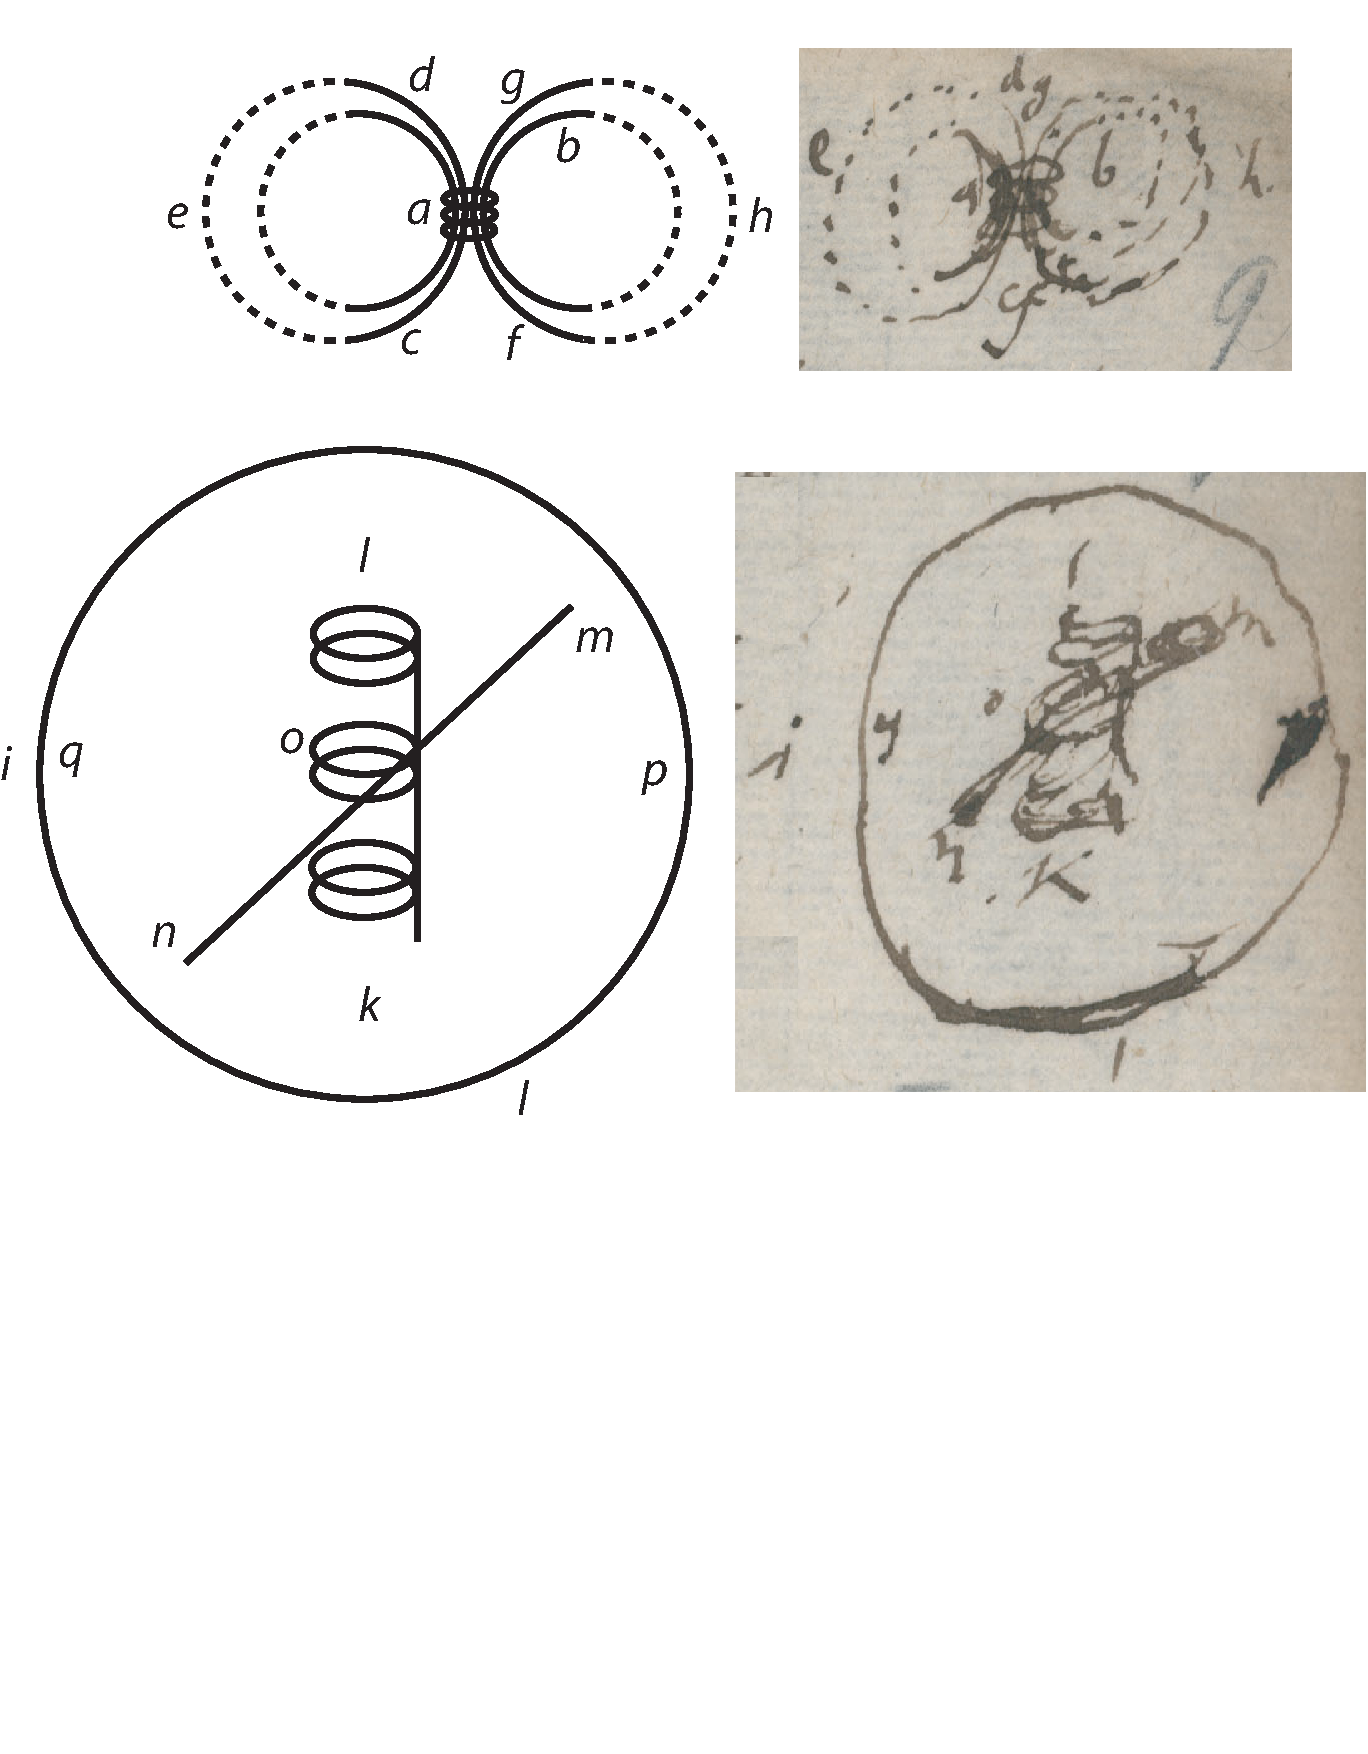
\includegraphics[trim = 0mm -3mm 0mm 0mm, clip, width=0.68\textwidth]{images/lh0040104b_009r1.pdf}\\
%\centering [\textit{Fig. 13}]%
%% \end{wrapfigure}%
%%
%\pend%
%\vspace*{1em}% PR: Rein provisorisch !!!
%\pstart%
%\noindent% PR: Neuer Abschnitt.
\edtext{In%
\edlabel{004_01_04b_009r_pU1a}%
\edtext{}{{\xxref{004_01_04b_009r_pU1a}{004_01_04b_009r_pU1b}}\lemma{In eo [...] deduci}\Cfootnote{Für diese Passage aus Descartes' verschollenem Ms. besteht eine paral\-lele Überlieferung in \cite{01144}\textsc{R.~Descartes}, \textit{Opuscula posthuma}, Amsterdam 1701, \glqq Primae co\-gi\-ta\-tio\-nes circa generationem animalium\grqq, S.~21f. Siehe \cite{00120}\textit{DO} XI, S.~534.13-535.21.}}
eo convenit}{\lemma{In eo convenit}\Cfootnote{%
Von hier an weitet sich die Thematik der Auszüge aus.
Den anatomischen Berich\-ten schließen sich physiologische und zum Teil auch medizinische Beobachtungen in höherem Maße an.}}
%
formatio plantarum et animalium quod fiant a partibus materiae vi caloris in
\edtext{orbem convolutae,}{\lemma{orbem}\Bfootnote{\textit{(1)}\ circumvolutae \textit{(2)}\ convolutae, \textit{L}}}
sed in hoc discrepant, quod partes materiae ex quibus plantae generantur volvuntur tantum in orbem circulariter;
eae vero ex quibus animalia volvantur sphaerice et in omnes partes.
Nam si v.g. partes materiae ex $a$ volvantur versus $b$ et $a$ per illas transeunt aliae partes ex $c.f$ versus $d.e.c.g.h.f.$
quarum $cf$ faciunt radices $dg$ ramos et folia $ab$ vero truncum plantae.
Si vero partes materiae $li$ volvantur sphaerice tunicam rotundam efficiunt
\edtext{[quae]}{\lemma{qui}\Bfootnote{\textit{L \"{a}ndert Hrsg.}}}
totum foetum involvit, ac proinde hic foetus non potest adhaerere terrae ut plantae.
Sed ita formatur 1\textsuperscript{o} materia in hac tunica sphaerica contenta
dum in orbem ibi circulatur transcendendo ex $l$ versus $k$ et inde circulariter in omnes partes ut $kpl,$ $kql,$ efficit tubum $lk$
qui repraesentat oesophagum;
praeterea partes subtiliores materiae istius cum non possint semper ita facile per istum canalem $lk$ transire
secedunt versus $m$ ubi cerebrum repraesentant;
crassiores vero utpote violentius agitatae versus $n,$ ubi hepar et lien efficiunt.
%\begin{wrapfigure}{r}{0.7\textwidth}
%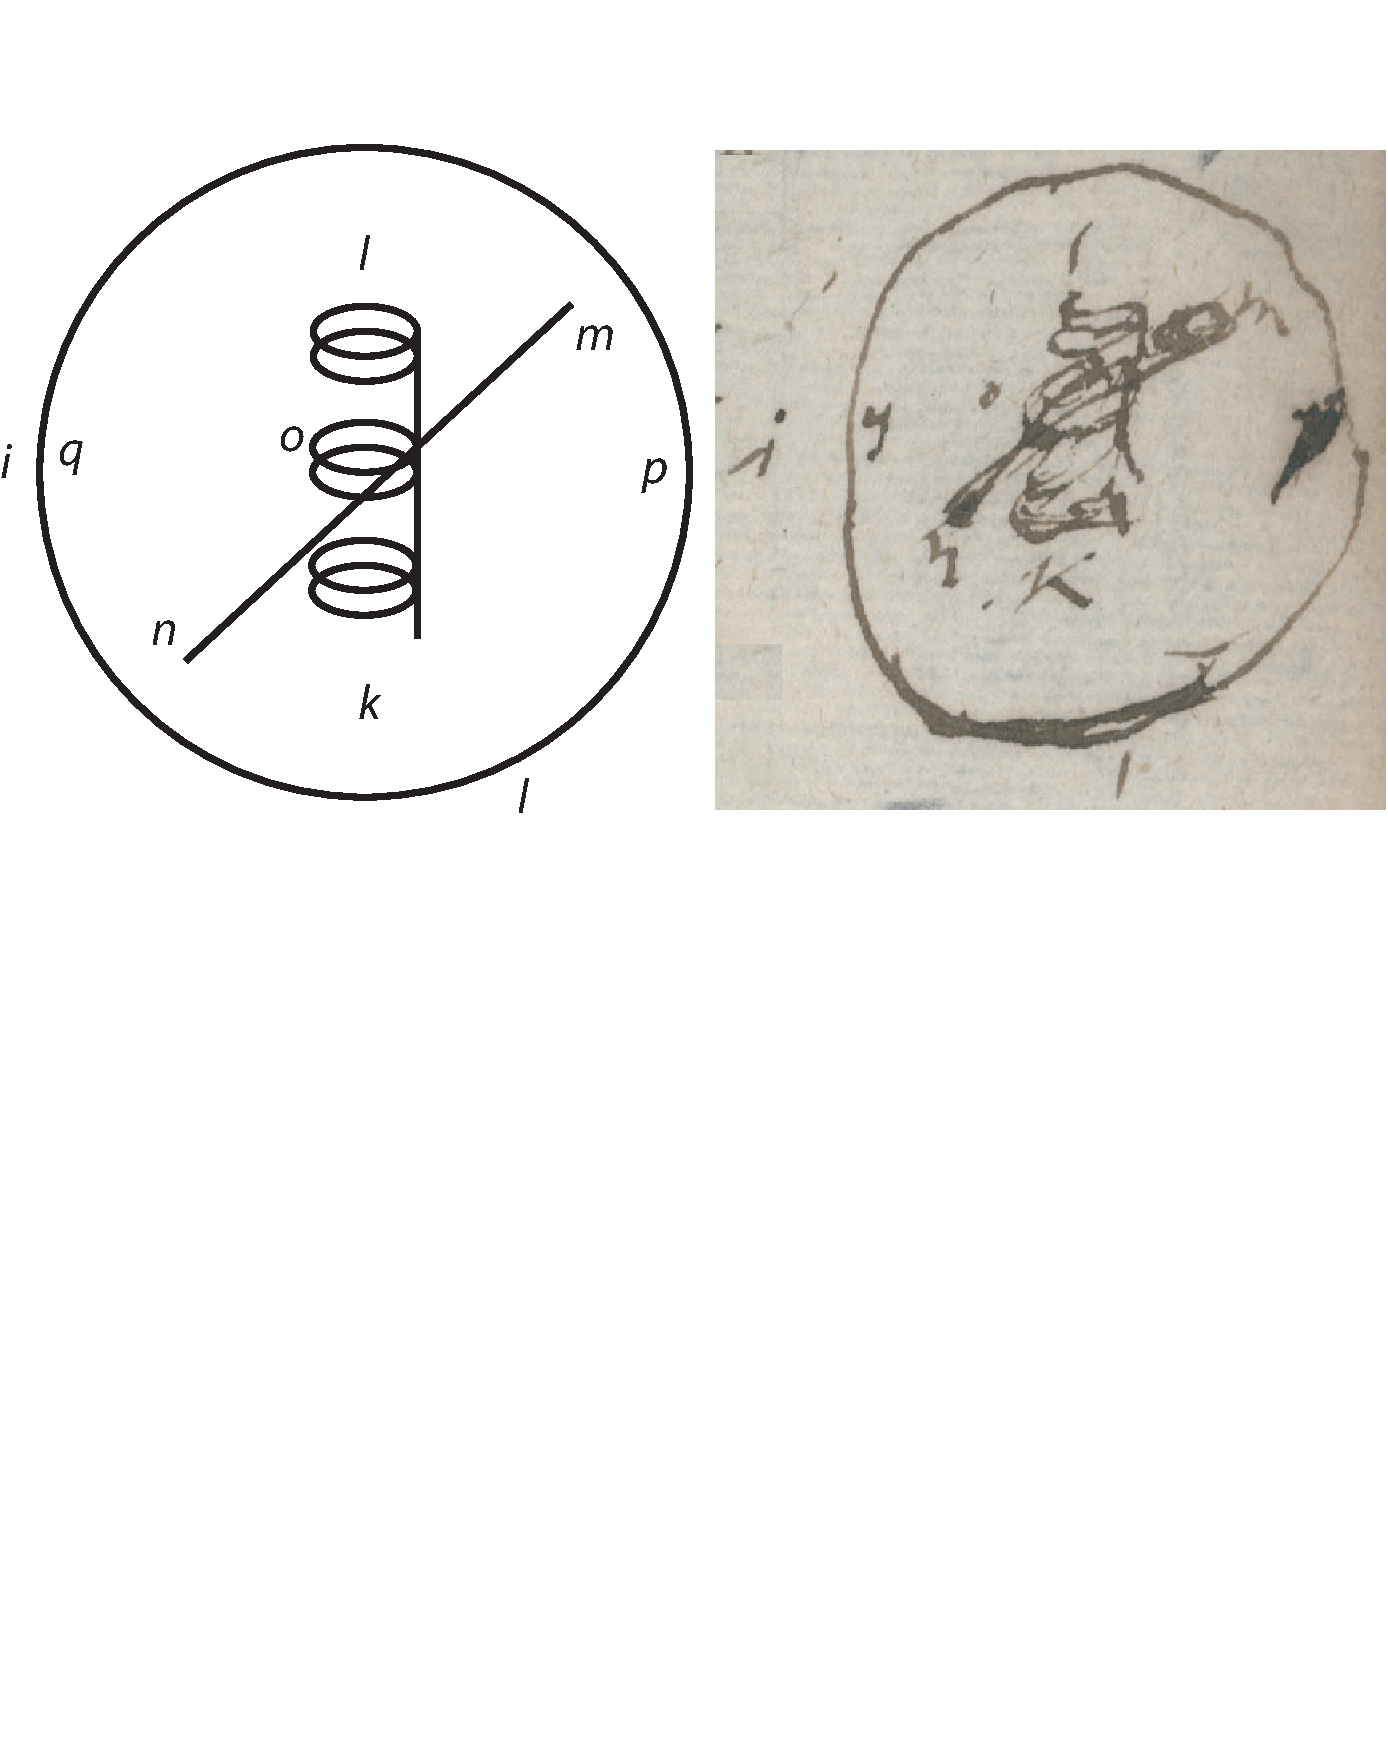
\includegraphics[width=0.7\textwidth]{images/lh0040104b_009r2.pdf}
%\caption{Bildbeschreibung}
%\end{wrapfigure}
Deinde redundantes spiritus ex cerebro efficiunt
\edtext{asperam arteriam}{\lemma{asperam}\Bfootnote{\textit{(1)}\ arteriosam \textit{(2)}\ arteriam \textit{L}}}
eique simul continuam venam arteriosam,
et e contra spiritus ex hepate redundantes \makebox[1.0\textwidth][s]{efficiunt cavam,
atque ex concursu cavae et venae arteriosae generatur cor versus $o$ in} medio corporis animalis;
hinc tres ventres in omnibus animalium, et caeterorum omnium membrorum \edlabel{004_01_04b_009r_pU1b}confirmatio facile potest \setline{16}deduci.%
%
\pend
%\newpage
\vspace{2.5em}
\pstart
\centering
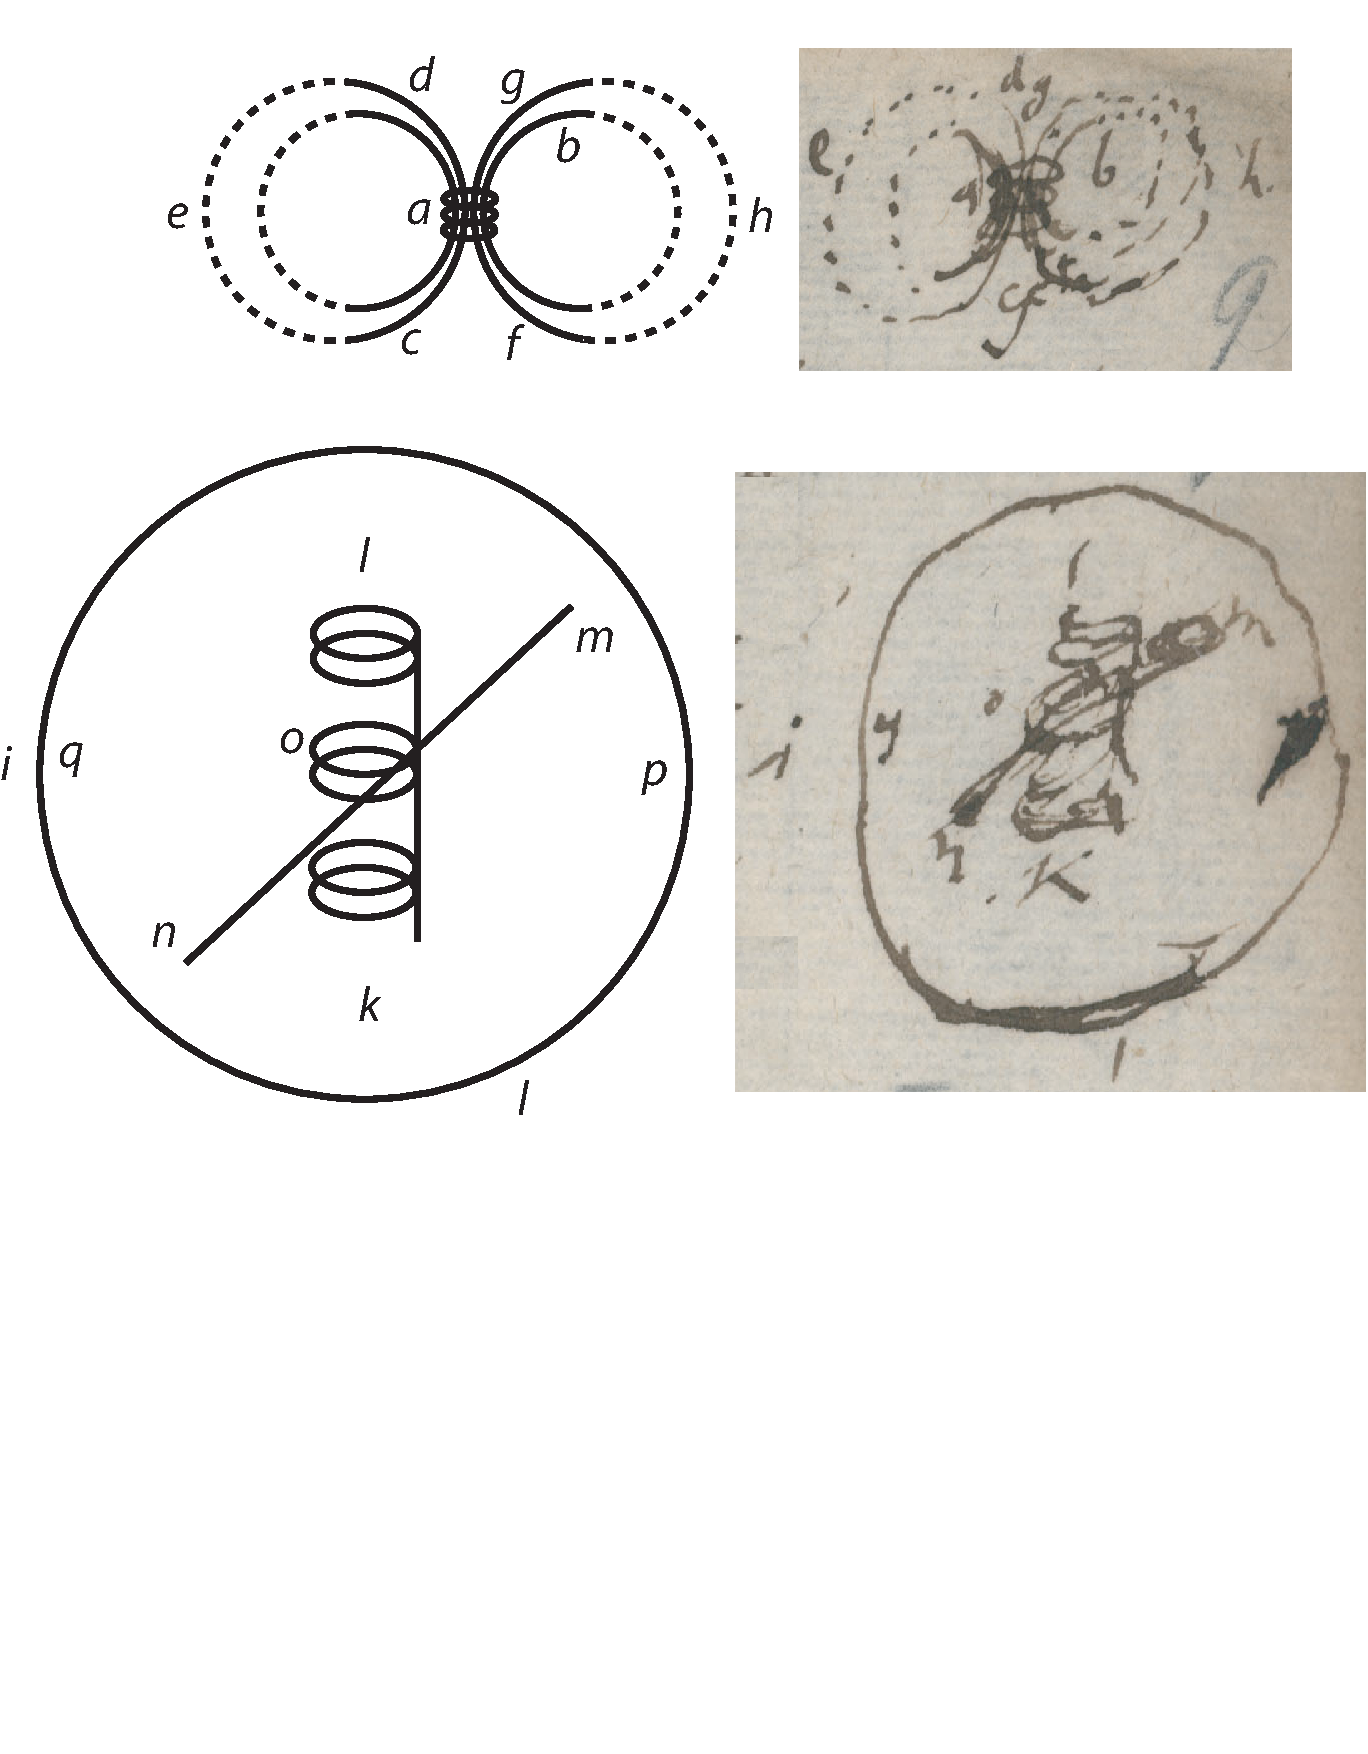
\includegraphics[trim = 0mm -3mm 0mm 0mm, clip, width=0.68\textwidth]{images/lh0040104b_009r1.pdf}\\
\centering [\textit{Fig. 13}]%
\pend
\count\Bfootins=1200
\newpage
\pstart
\edtext{[Laetitia]}{\lemma{Laetitita}\Bfootnote{\textit{L \"{a}ndert Hrsg.}}}
et tristitia possunt effici ex solo sensu cordis nullo habito respectu ad res externas amor vero est ad bonum externum et odium ad malum praesens vel elapsum,
et metus ad malum impendens et desiderium ad bonum acquisibile, et ira ad injustitiam ab alio factam etc.
\pend%
\pstart%
Frigemus\edlabel{004_01_04b_009r_pU2a}%
\edtext{}{{\xxref{004_01_04b_009r_pU2a}{004_01_04b_009r_pU2b}}\lemma{Frigemus [...] intermissis}\Cfootnote{Für diese Passage aus Descartes' verschollenem Manuskript besteht eine pa\-ral\-lele Überlieferung in \cite{01144}\textsc{R.~Descartes}, \textit{Opuscula posthuma}, Amsterdam 1701, \glqq Primae co\-gi\-ta\-tio\-nes circa generationem animalium\grqq, S.~22. Siehe \cite{00120}\textit{DO} XI, S.~535.22-537.8.}}
statim a cibo cum recte valemus,
quod tunc ciborum succus recta per venas ingrediens massam sanguinis illam totam refrigerat,
et tunc minus loci occupans confluit versus cor et deserit extremitates membrorum, quae ideo magis frigent,
eodem modo fit in febre, quod humor febrem causans sanguini se immiscet,
et ingrediens cor ejus ignem imminuit, postea tamen auget et sic omnia membra calefacit
(+ necesse est hunc succum esse quodammodo inflammabilem, sed cum difficultate +)
ut aqua carbonibus injecta initio quidem extinguit, sed statim rursus inflammati magis ardent.
Non semper autem frigemus statim a cibo, quod non semper ita confestim succi ciborum venas ingrediuntur,
vel etiam illi succi non refrigerant sanguinem,
quin imo etiam aliqui efficiunt ut sudemus praesertim in fronte, ut acetum,
quod scilicet cor ingredientes ibi magis inflammantur, et statim evolant versus caput;
fierique potest ut eodem tempore cibus efficiat, ut fronte sudemus et extremitatibus frigeamus.
\pend%
\pstart%
In sanguine quatuor sunt praecipua genera partium tenues et laeves ut spiritus vini;
tenues et ramosae, ut olea, crassae et laeves ut aquae et salia, crassae et ramosae ut terra vel cineres.
Tenues et laeves faciunt ephemeram febrim, retentae et putrescentes in extremitatibus vasorum, ob defectum insensibilis transpirationis.
Crassae et laeves faciunt febrem quotidianam putrescentes in stomacho et intestinis;
tenues et ramosae faciunt tertianam putrescentes in cysti fellis, crassae et ramosae faciunt quartanam, in liene putrescentes;
putrefactio autem humoris et adhaesio,
et reactio partium ejus ad partes parum distantes, quae putrefactio cordis igne discutitur,
et ita cum humor pervenit ad venas fit accessio (+ acc\`{e}s +) paulatimque discutitur.
Exonerat autem se cystis fellis in ventriculum et intestina atque inde in venas alternis diebus, lien vero 2 diebus intermissis.%
\edlabel{004_01_04b_009r_pU2b}%
\pend%
\vspace{0.7em}% PR: Diesen leeren Zeilenabstand bitte behalten !!!
\pstart%
\noindent% Neuer Abschnitt.
\textso{De accretione et nutritione, 1637. Nov. }%
Accretio duplex est alia mortuorum et quae non nutriuntur, fitque per simplicem partium appositionem sine
\edtext{ulla earum immutatione,}{\lemma{ulla}\Bfootnote{\textit{(1)}\ partium immutatione \textit{(2)}\ earum immutatione, \textit{L}}}
vel saltem sine magna; ita crescunt metalla in fodinis, ita mel in apiariis etc. absque ulla partium mutatione: ita crescunt etiam lapides
\edtext{et similia}{\lemma{et similia}\Bfootnote{\textit{erg. L}}}
sine magna partium mutatione, (vel etiam cum magna nihil vetat) et fit etiam transmutatio ligni vel alterius corporis in lapidem per modum talis accretionis,
dum partes lapidis poros ligni ingrediuntur, et praecedentes vel sibi assimilant vel extradunt; vel partim hoc partim illud.
\pend%
\pstart%
Alia accretio est viventium sive eorum quae nutriuntur, et fit semper cum aliqua partium immutatione.
Nempe partes variae variarum figurarum sibi mutuo occurrentes miscentur et ita permixtae in se mutuo agunt,
donec quasdam determinatas figuras acquirant.
Interdumque fluidiores ex his elabuntur, minus fluidis manentibus quae unae aliis impactae durum corpus componunt
per quod rivuli omnibus simul mixtis repleti varii ubique excurrunt et crassiores partes illis rivulis contentae in locum circumjacentium
paulatim succedunt pulsae a tenuioribus, atque ita fit nutritio:
vel rivulum unum in duos aut plures dividunt atque ita fit accretio;
nempe corpus ita crescens innummeris ejusmodi rivulis est refertum;
et cum ob senectutem partes duriores ita impactae sunt ut rivuli illis circumsepti non dilatari amplius possint,
ut ex uno duo fiant cessat accretio,
manetque tantum nutritio quod si deinde successu temporis istae partes crassiores adhuc magis compingantur,
ut ab aliis advenientibus loco pelli non possint, cessat etiam nutritio et vita.
\pend%
\count\Bfootins=1200
%\count\Cfootins=1500
%\count\Afootins=1500
\pstart%
Est autem haec accretio sive nutritio vel imperfecta vel perfecta.
Imperfecta est cum materia illos rivulos replens aliunde advenit jam ita permixta vel proxime, disposita ut ita misceatur et formetur, et ita nutriuntur pili, ungues, cornua, fungi, tuberes, partesque omnes tum animalium, tum plantarum, itemque plantae quodam semine carentes, et forte etiam animalia imperfectissima, ut ostreae quae simile non generant.
Perfecta nutritio sive accretio simul generationem sive seminis productionem continet et fit quando materia rivos replens est talis, ut aliam advenientem (non quidem absolute quamlibet, hoc enim vix unquam posset contingere, sed quamlibet non nimis contumacem et diversae naturae) sibi possit omnino assimilare, ita scilicet, ut si constet exempli causa particulis trium generum tantum nempe perexiguis prismatibus, paulo majoribus conoidibus, et aliis certo modo ad has duas simul jungendas apto, concavis, ex omni materia quae tris miscebitur, fiant rursus quaedam prismata conoidea, et partes concavae his simul jungendis aptae, nec tamen repugnat quin simul ex eadem materia varia alia partium genera emergant ut semper vel fere semper accidit, sed hae tres solae existentes semen componunt aliis vero diversimode conjunctae, vel etiam aliae
\edtext{novae}{\lemma{novae}\Bfootnote{\textit{erg. L}}}
sine ipsis componunt lignum, corticem, radices, folia, flores, fructus, etc. in plantis; idemque in animalibus carnes, ossa, cerebrum, \makebox[1.0\textwidth][s]{membranas, sanguinem etc.
Potest % Hier endet Bl. 9r un beginnt Bl. 9v.
[9~v\textsuperscript{o}]
vero etiam contingere ut partes seminis non}
\pend
\newpage